\section{Simulación de esqueletos} \label{sec_esqueletos}
%el Modelo de Mezcla Gaussiana visto en la sección \ref{sec_GMM}.
En esta sección vamos a explicar cómo generamos la matriz \textit{mat\_esqueleto}, utilizando la metodología $B$ seleccionada en la sección anterior. La matriz tiene $t$ renglones y $m$ columnas. En la entrada $(h,j)$ tiene el número de grupos simulados para la hora $h$ y la materia $j$. La matriz \textit{mat\_esqueleto} depende de la demanda de alumnos y de las solicitudes de los profesores.


Los pasos que seguimos para obtener la matriz \textit{mat\_esqueleto} con la metodología $B$ son:

\begin{enumerate}
\item Definir \textit{n\_rep}, el número de veces que se va a generar la matriz $D'_{n}$ con la demanda de alumnos para el siguiente semestre.

\item Simular $D'_{1}$ con la función \textit{gen\_mat\_demanda\_alumnos} (ver Sección \ref{SimDemandaAlumnos}).

\item Definir la matriz \textit{prom\_D} igual a $D'_{1}$. La matriz \textit{prom\_D} guardará el número de alumnos simulados promedio.

\item Simular \textit{mat\_solicitudes} con la función \textit{gen\_solicitudes} (ver Sección \ref{SimSolicitudesProfesores}).

\item Simular un esqueleto inicial con la función \textit{gen\_esqueleto} (ver Subsseción \ref{subsec_gen_esqueleto}).

\item Guardar el número de grupos por materia.

\item Convertir y guardar los datos del esqueleto inicial para obtener la distribución por horas (\textit{wait\_mat\_esqueleto}).

\item Graficar los datos del esqueleto inicial para ver su distribución. Con esta gráfica encontrar el número de medias inicial, en nuestro caso $k = 4$ (ver \figurename{~\ref{hist_wait_esq_ini}}).

\item Definir el modelo inicial \textit{mixmdl\_1\_esqueleto} con la función de \textit{R}:

\verb@normalmixEM(wait_mat_esqueleto,k = 4)@.
\end{enumerate}

\begin{figure}[H]
\centering
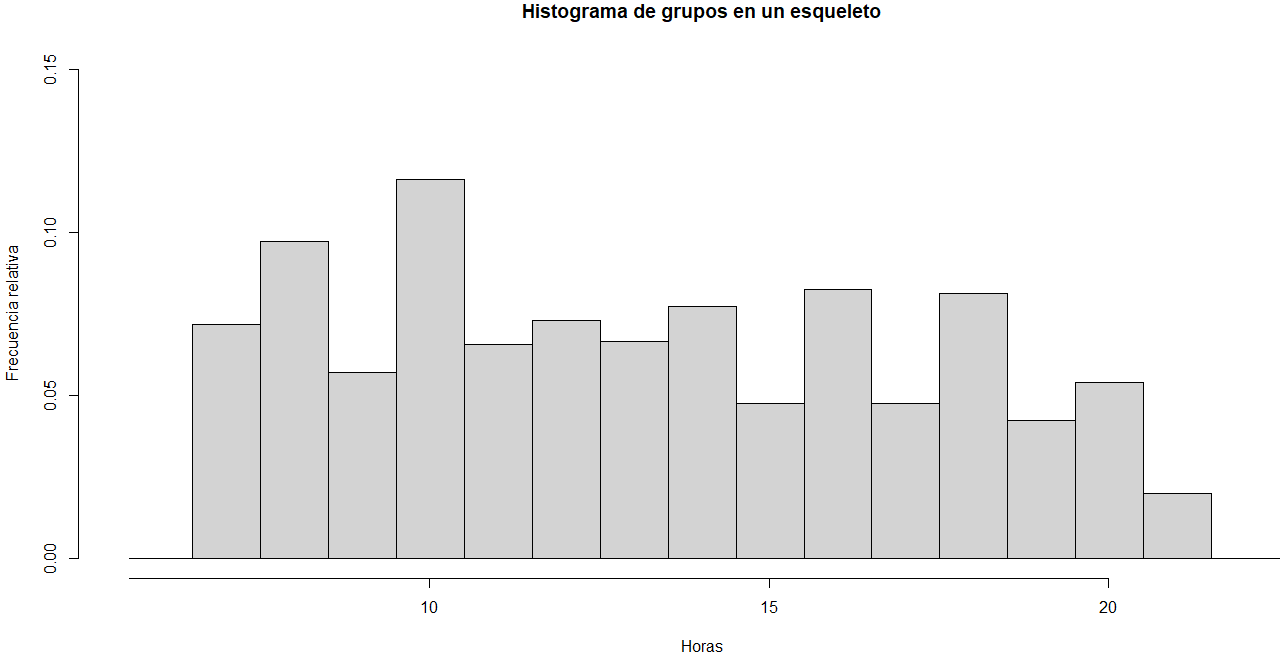
\includegraphics[width=\textwidth]{hist_wait_esqueleto_inicial} %scale = 0.7
\caption[\textit{Histograma con los datos del esqueleto inicial}]{\textit{Se muestra el histograma con los datos del esqueleto inicial.}}\label{hist_wait_esq_ini}
\end{figure}


Pasos a repetir $(n = 2, \ldots, \textit{n\_rep})$:

\begin{enumerate}
\item Obtener $D'_{n}$ con la función \textit{gen\_mat\_demanda\_alumnos}.

\item Definir \textit{prom\_D} = \textit{prom\_D} + $D'_{n}$.

\item Simular \textit{mat\_solicitudes} con la función \textit{gen\_solicitudes}.

\item Simular un esqueleto con la función \textit{gen\_esqueleto}.

\item Guardar el número de grupos por materia.

\item Convertir y guardar los datos del esqueleto en el vector \textit{wait\_mat\_esqueleto}.
\end{enumerate}

Pasos finales:

\begin{enumerate}
\item Calcular el promedio de grupos por materia. Para ello, aplicar las siguientes funciones de \textit{R}, a la matriz \textit{prom\_D}: \verb@ceiling(colMeans((prom_D))@ 

\item Definir el modelo final \textit{mixmdl\_esqueleto} con la función en \textit{R} (ver \figurename{~\ref{hist_wait_esq_fin}}):

\verb@normalmixEM(wait_mat_esqueleto,k = 4,mean=mixmdl_1_esqueleto$mu)@.

\item Generar la matriz \textit{mat\_esqueleto} en base al promedio obtenido y a la distribución del modelo final. Por ejemplo, si se tiene una materia con 5 grupos simulados, entonces se simulan 5 números aleatorios con distribución Normal. El comando en \textit{R} es: \verb@round(rnorm(5,mixmdl_esqueleto$mu,mixmdl_esqueleto$sigma))@
\end{enumerate}
 
\begin{figure}[H]
\centering
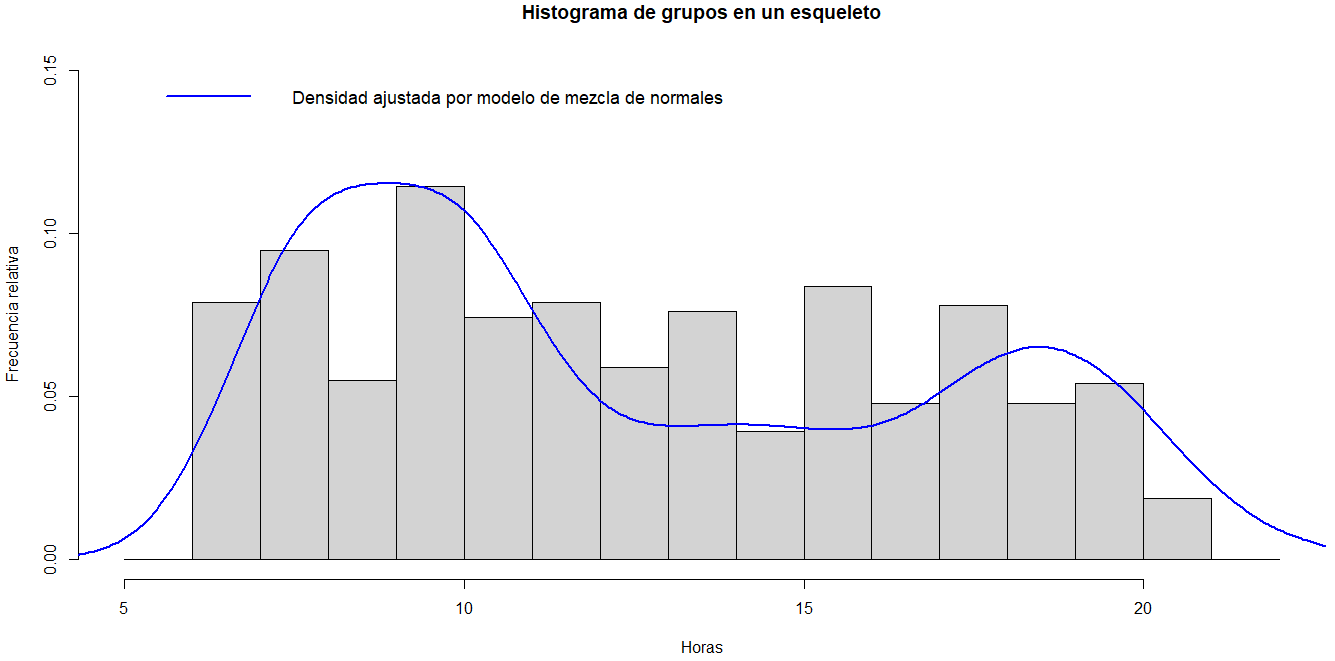
\includegraphics[width=\textwidth]{hist_wait_esqueleto_final} %scale = 0.7
\caption[\textit{Histograma con los datos del esqueleto final}]{\textit{Se muestra el histograma con los datos del esqueleto final. La línea azul representa la distribución ajustada por el modelo final.}}\label{hist_wait_esq_fin}
\end{figure}


En la \figurename{~\ref{esqueleto20202}} vemos un ejemplo de la matriz \textit{mat\_esqueleto} para el semestre 2020-2. Observemos las últimas 4 columnas que corresponden a las materias de \textit{Cálculo Diferencial e Integral I, II, III} y \textit{IV}. Notamos que el número de grupos simulados para \textit{Cálculo Diferencial e Integral II} es mayor a al número de grupos de \textit{Cálculo Diferencial e Integral I}.Esto se debe al comportamiento descrito en la Sección \ref{AE_x_GpoDeDatos} y el semestre 2020-2 es par. Para \textit{Cálculo Diferencial e Integral III} y \textit{IV} el número de grupos simulados es prácticamente igual.

\begin{figure}[H]
\centering
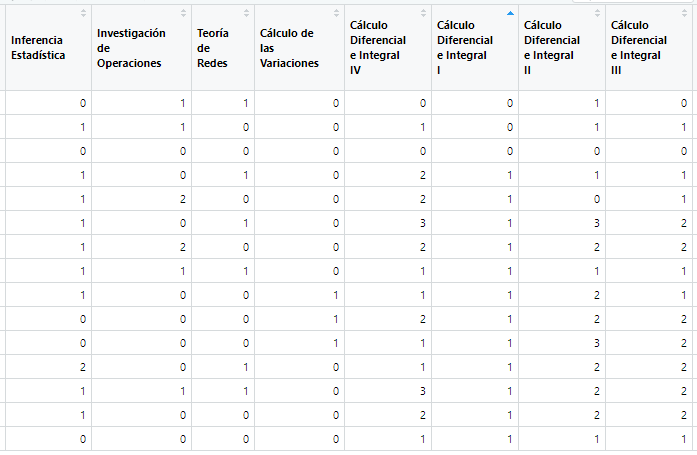
\includegraphics[width=\textwidth]{Ej_esqueleto_20202} %scale = 0.7
\caption[\textit{Ejemplo de esqueleto para el semestre 2020-2}]{\textit{Ejemplo de esqueleto para el semestre 2020-2: En la entrada (i,j) podemos observar el número de alumnos simulados para la hora i y la materia j.}}\label{esqueleto20202}
\end{figure}


%\textbf{NOTAS:}
%
%\begin{itemize}
%\item[-] Sólo estamos haciendo operaciones cuando las entradas de \textit{bin\_DUE} haya un 1.\\
%
%\item[-] La diferencia relativa la definimos como $\dfrac{D - E}{D}$ porque la demanda es lo que esperamos que ocurra.
%\end{itemize}
%
%En la \figurename{~\ref{dif_D_E_gpo}} vemos el histograma de la diferencia de las matrices D - E. Diferencia entre el número de alumnos esperados menos el número de alumnos simulados por grupo. Los valores se encuentran entre -166 y 432.
%
%\begin{figure}[H]
%\centering
%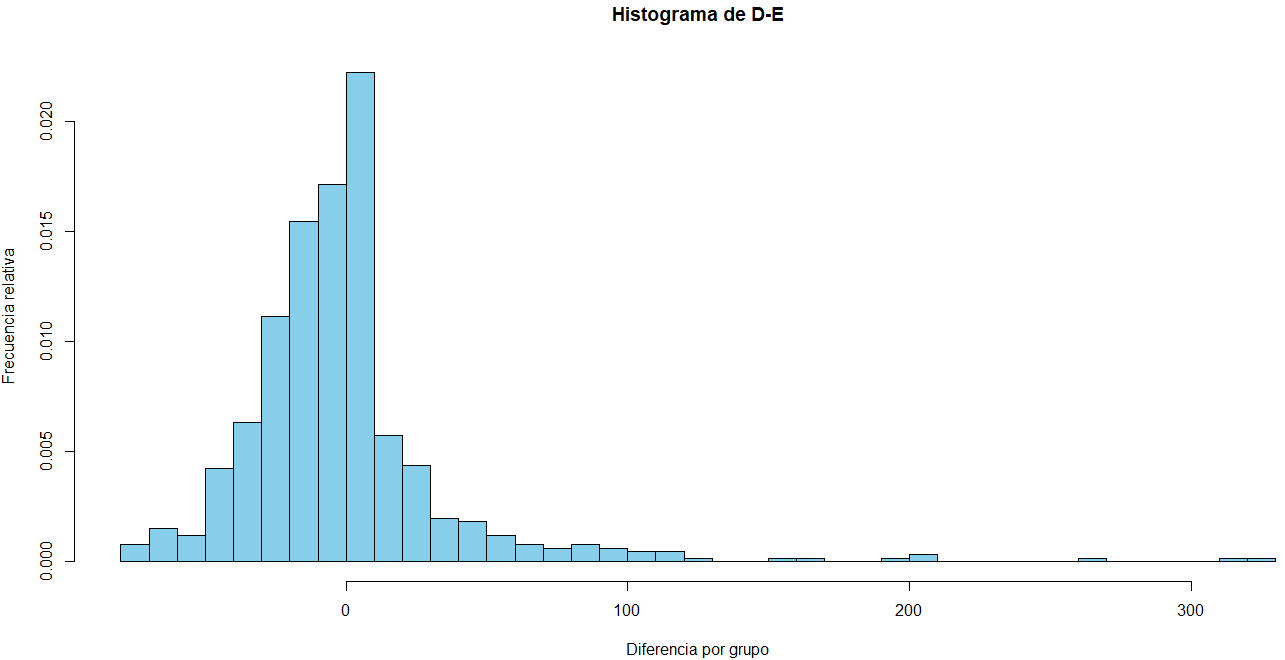
\includegraphics[scale = 0.5]{histograma_FR_D-E_x_gpo} %width=\textwidth
%\caption{\textit{Histograma de la diferencia de las matrices D - E por grupo}}\label{dif_D_E_gpo}
%\end{figure}
%
%
%En la \figurename{~\ref{difRel_D_E_gpo}} vemos el histograma de la diferencia relativa de las matrices D y E. Diferencia entre el número de alumnos esperados menos el número de alumnos simulados, entre el número de alumnos esperados, por grupo. Los valores se encuentran entre -71 y 1.
%
%El valor de -71 corresponde a la materia \textit{Teoría de los Conjuntos I}. A las 14hrs, en la matriz D vale 1 y en la matriz E vale 72 entonces el error relativo es -71.
%
%El valor de -64 corresponde a la materia \textit{Inferencia Estadística}. A las 12hrs, en la matriz D vale 1 y en la matriz E vale 65 entonces el error relativo es -64.
%
%El valor de -61 corresponde a la materia \textit{Probabilidad II}. A las 11hrs, en la matriz D vale 1 y en la matriz E vale 62 entonces el error relativo es -61.
%
%El valor de -61 corresponde a la materia \textit{Historia de las Matemáticas I}. A las 13hrs, en la matriz D vale 1 y en la matriz E vale 62 entonces el error relativo es -61.
%
%El valor de -50 corresponde a la materia \textit{Demografía}. A las 17hrs, en la matriz D vale 1 y en la matriz E vale 51 entonces el error relativo es -50.
%
%El valor de 1 corresponde a 111 materias, veamos 5 casos: \textit{Álgebra Moderna I (8hrs), Álgebra Lineal II (8hrs), Análisis Matemático II (16hrs), Manejo de Datos (16hrs), Seminario sobre enseñanza de las Matemáticas I (17hrs)}. En la matriz D valen 6, 16, 21, 3 y 7 respectivamente. En la matriz E valen 0, entonces el error relativo es 1.
%
%\begin{figure}[H]
%\centering
%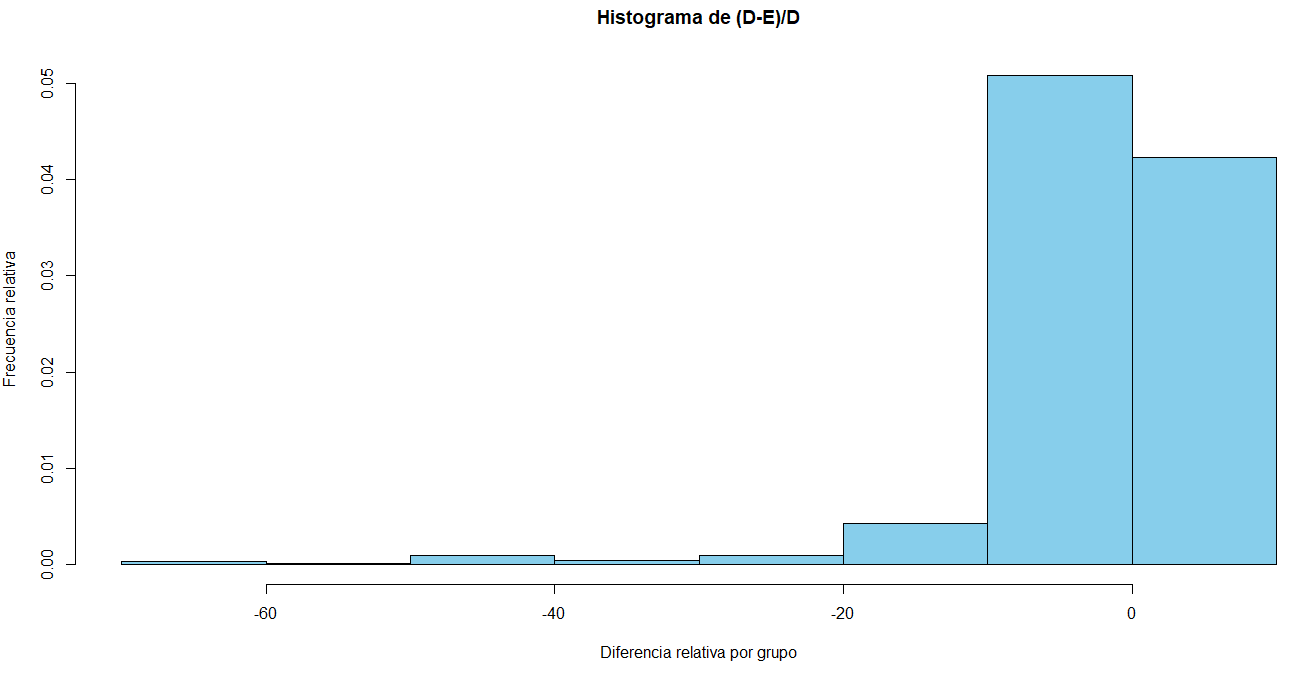
\includegraphics[scale = 0.5]{histograma_FR_D-E_D_x_gpo} %width=\textwidth
%\caption{\textit{Histograma de la diferencia relativa de las matrices D y E por grupo}}\label{difRel_D_E_gpo}
%\end{figure}


%En la \figurename{~\ref{dif_D_E_materia}} vemos el histograma de la diferencia de las matrices D - E. Diferencia entre el número de alumnos esperados menos el número de alumnos simulados por materia. Los valores se encuentran entre -259 y 244.
%
%\begin{figure}[H]
%\centering
%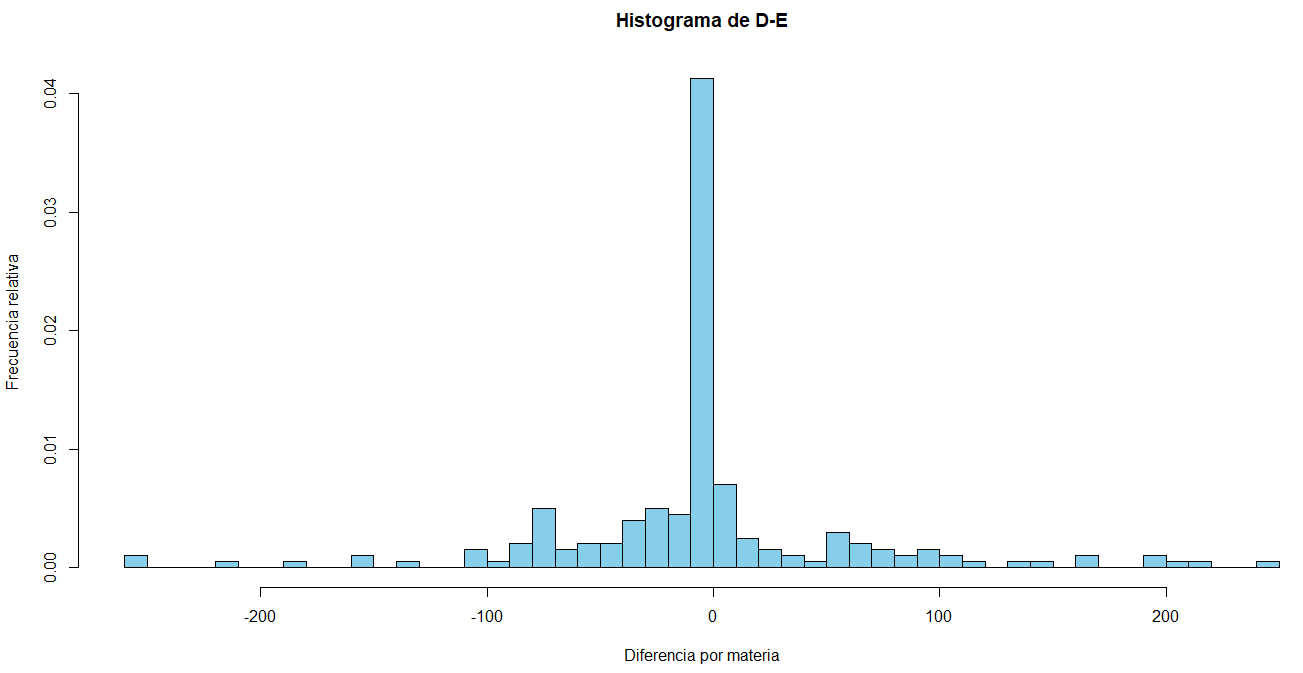
\includegraphics[scale = 0.4]{histograma_FR_D-E_x_materia} %width=\textwidth
%\caption{\textit{Histograma de la diferencia de las matrices D - E por materia}}\label{dif_D_E_materia}
%\end{figure}

%
%En la \figurename{~\ref{difRel_D_E_materia}} vemos el histograma de la diferencia relativa de las matrices D y E. Diferencia entre el número de alumnos esperados menos el número de alumnos simulados, entre el número de alumnos esperados, por grupo. Los valores se encuentran entre -97 y 6.
%
%\begin{figure}[H]
%\centering
%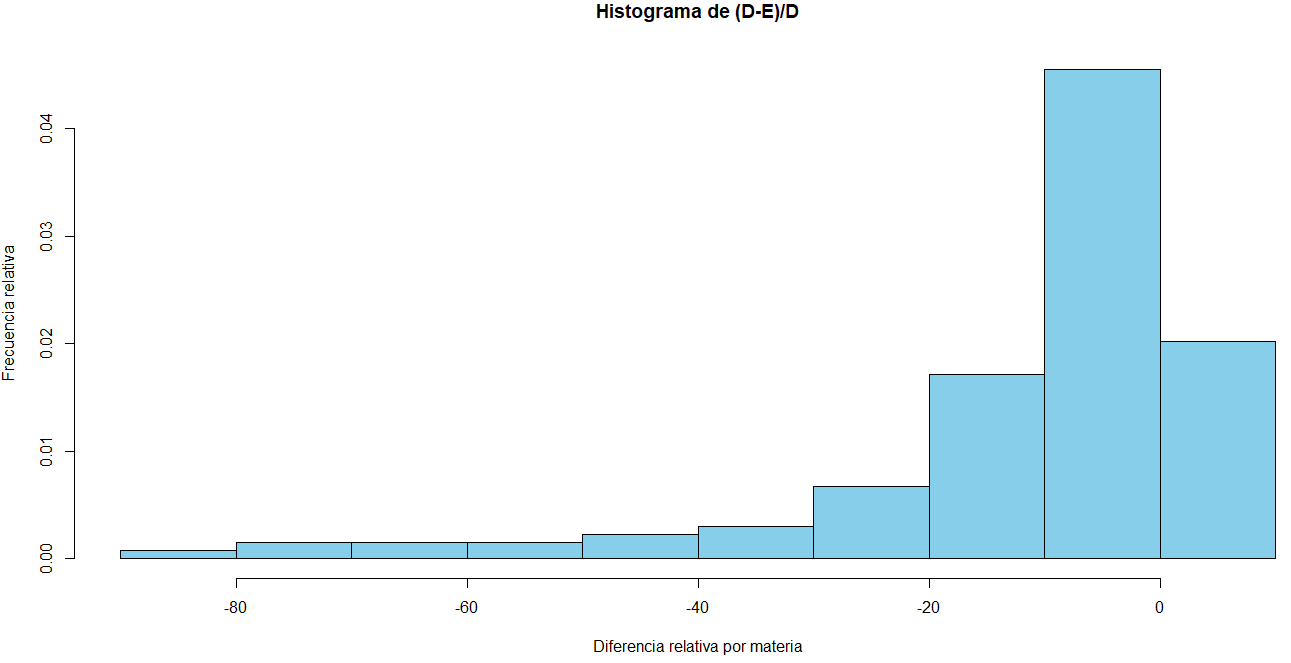
\includegraphics[scale = 0.4]{histograma_FR_D-E_D_x_materia} %width=\textwidth
%\caption{\textit{Histograma de la diferencia relativa de las matrices D y E por materia}}\label{difRel_D_E_materia}
%\end{figure}
%
%En la siguiente figura vemos las 20 materias con error relativo más negativo:
%
%\begin{figure}[H]
%\centering
%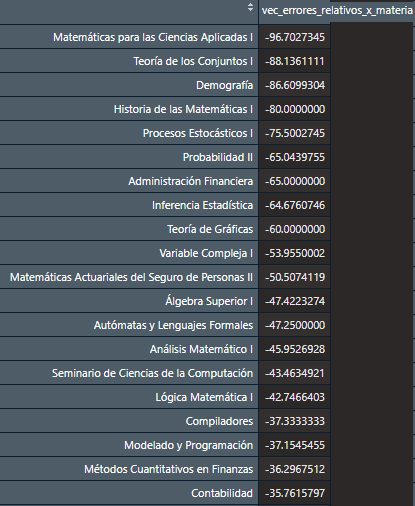
\includegraphics[scale = 1]{error_relativo_20materias_negativo} %width=\textwidth
%\caption{\textit{error relativo 40materias}}
%\end{figure}
%
%En la siguiente figura se tienen los valores en D y E de los 5 casos más negativos:
%
%\begin{figure}[H]
%\centering
%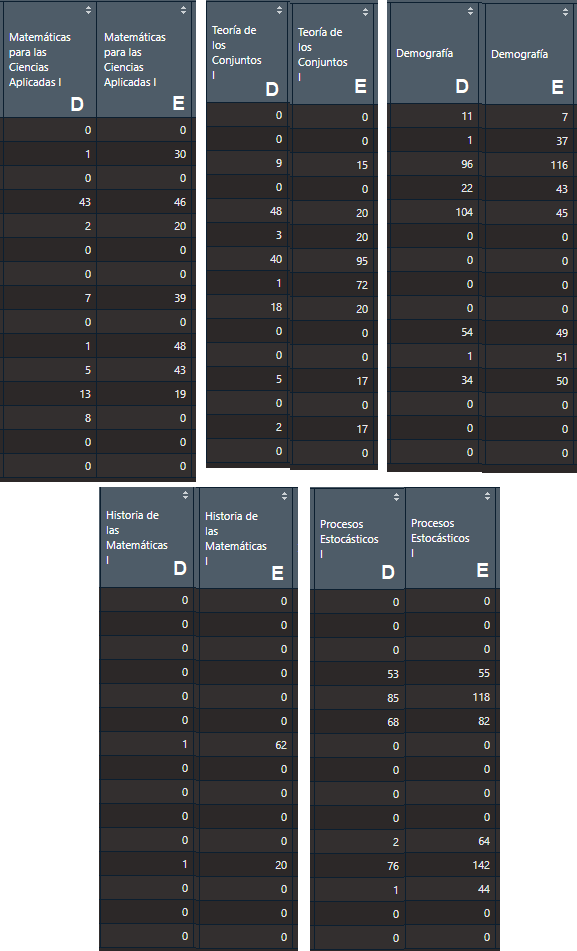
\includegraphics[scale = 0.85]{D_E_5_negativos} %width=\textwidth
%\caption{\textit{Casos más negativos}}
%\end{figure}
%
%
%En la siguiente figura vemos las 20 materias con error relativo más positivo:
%
%\begin{figure}[H]
%\centering
%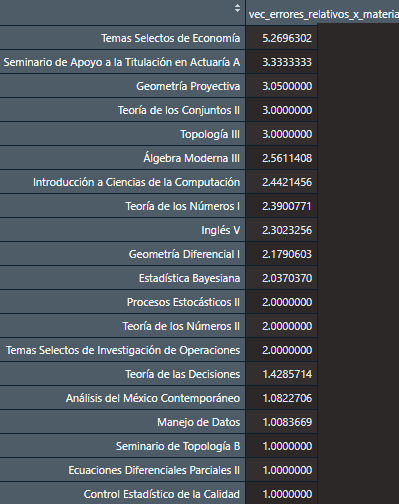
\includegraphics[scale = 1]{error_relativo_20materias_positivo} %width=\textwidth
%\caption{\textit{error relativo 40materias}}
%\end{figure}
%
%En la siguiente figura se tienen los valores en D y E de los 5 casos más positivos:
%
%\begin{figure}[H]
%\centering
%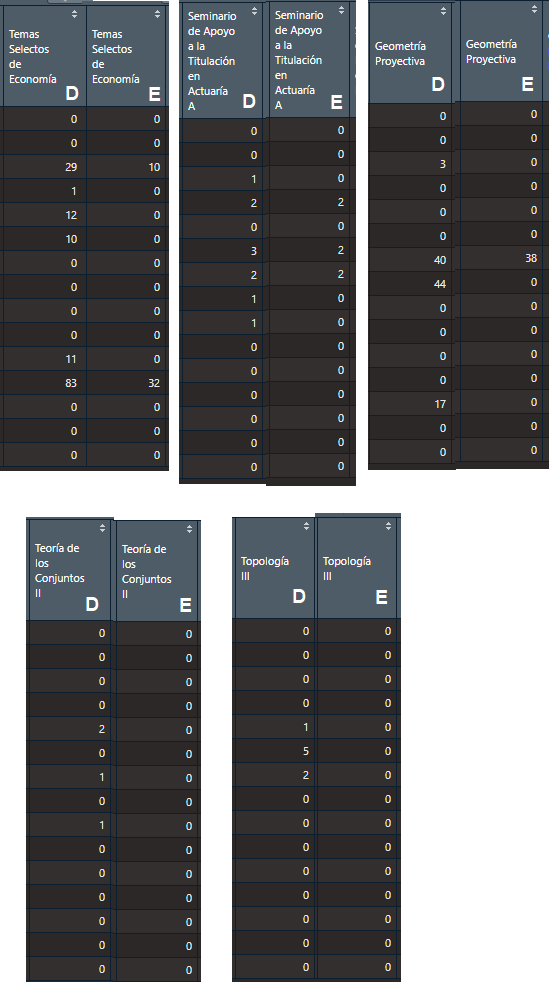
\includegraphics[scale = 0.9]{D_E_5_positivos} %width=\textwidth
%\caption{\textit{Casos más positivos}}
%\end{figure}
%
%
%\begin{eqnarray*}
%L_{materia} &=& -1 \,\,\,\,\,\,  \text{por cada materia no impartida}\\
%x &=& \text{promedio}\\
%y &=& \text{cupo}\\
%L_{dif\_p\_c} (x,y) &=& \begin{cases}
%\dfrac{a}{190} (x-y)  & \quad \text{si } x<y\\
%- \dfrac{b}{190} (x-y)  & \quad \text{si } x\geqslant y
%\end{cases}\\
%a &=& 0.5\\
%b &=& 0.8\\
%L_{categoria}^{1} (mat,solicitud) &=& -c(categoria - 1)\\
%L_{categoria}^{2} (mat,solicitud) &=& -c_{1}(categoria)
%\end{eqnarray*}
%
%Al momento de simular las solicitudes de materias para los profesores suponemos que la que está en primer lugar es la materia que más quiere dar, en segundo lugar, la segunda que quiere dar.
%
%Primero asignar grupos a los profesores de tiempo completo. Después asignar grupos faltantes a los profesores de asignatura.
%
%$L_{materia}$ es la penalización por no tener en el esqueleto una materia que necesitamos.
%
%$L_{dif\_p\_c}$ es la penalización en la asignación de salones. Se tiene un grupo de tamaño $x$ y un salón con capacidad $y$. Se penaliza con $\dfrac{a}{190}$ veces la diferencia entre $x$ y $y$ cuando el tamaño del grupo es menor a la capacidad del salón y se penaliza con $-\dfrac{b}{190}$ veces la diferencia entre $x$ y $y$ cuando el tamaño del grupo es mayor a la capacidad del salón.
%
%El esqueleto depende de la demanda de alumnos y de las solicitudes de los profesores.
%
%Primero se asignan materias a los profesores de tiempo completo y después a los de asignatura.
%
%Los profesores de asignatura pueden quedarse sin materias asignadas.
%
%Penalizaciones:
%  
%  \begin{enumerate}
%\item Si algún profesor pidió alguna materia y no se la dieron.
%
%\item Si hay alumnos que necesitan una clase a alguna hora y no existe profesor que la imparta.
%
%\item Con $\alpha \times num\_alumnos\_faltantes$ por cada alumno que te faltó en cada hora-materia que tenías que dar. $\alpha > 0$
%  
%  \item Con $\beta \times num\_alumnos\_sobrantes$ por cada alumno que te pasaste en cada hora-materia que tenías que dar. $\beta > 0$
%  
%  \end{enumerate}
%
%%Queremos el esqueleto con el menor valor en $\alpha + \beta$
%  
%  Con esto se califica un esqueleto.

\subsection{Función gen\_esqueleto} \label{subsec_gen_esqueleto}

Considerando que ya se generaron las matrices $D'$ y \textit{mat\_solicitudes}, el proceso que seguimos para obtener un esqueleto con la función \textit{gen\_esqueleto} es el siguiente:
  
  \begin{enumerate}
%\item Obtener la matriz \textit{mat\_demanda\_alumnos} con la demanda simulada del número de alumnos para el siguiente semestre (ver Sección \ref{GMM_D}).
%
%\item Obtener la matriz \textit{mat\_solicitudes} con las solicitudes simuladas de los profesores (ver Sección \ref{SimSolicitudesProfesores}).

\item Elegir un profesor de tiempo completo al azar.

\item Elegir al azar un horario y una materia que haya solicitado el profesor elegido en el paso anterior. Con estos datos obtenemos las coordenadas $(i,j)$ para las matrices $D'$ y \textit{mat\_esqueleto}.

\item Verificar que a esa materia en esa hora aún le sobran alumnos, en la entrada $(i,j)$ de $D'$.

\item Simular el número de alumnos para ese grupo (ver Sección \ref{SimTamGpos}).

\item Restar el número de alumnos simulados en el paso anterior, de la materia y hora elegidas, en la entrada $(i,j)$ de $D'$.

\item Ese profesor ya no puede impartir clases a esa hora. Retirar renglones correspondientes de \textit{mat\_solicitudes}.

\item Repetir los pasos de 1 a 6 hasta que se terminen los profesores.

\item Una vez que se terminen los profesores de tiempo completo, hacer los pasos de 1 a 7 con los profesores de asignatura.
\end{enumerate}

Algunas notas a considerar del procedimiento son:
  
  \begin{itemize}
%\item[-] Se le da prioridad de asignación a los profesores de tiempo completo.

\item[-] Los profesores de tiempo completo deben cumplir con sus horas, por contrato.

\item[-] Los profesores sólo pueden tener asignadas a lo más 2 materias.

\item[-] Las condiciones de paro del proceso son:
  
  \begin{itemize}
\item[a)] Ya se cubrió toda la demanda

\item[b)] Ya no hay más profesores

\item[c)] Llegar a una cota predefinida para que el ciclo no se haga infinito o tarde mucho en cumplir las condiciones anteriores.
\end{itemize}
\end{itemize}